% HK to edit
\section{Task Description}
\label{section_task}

Hungry Geese is a Kaggle simulation game, where each participant submit agents that compete with other agents. The rating of the team is the rating of its top agent.

In Hungry Geese, the main objective of each agent, or geese, is to survive. Similar to the Snake game popularised by Nokia phones, eating food will extend the length of the geese, and bumping to any agent will result in death.

% Statement: \textbf{Training a bot to obtain a high score in the Kaggle Competition}
% \\[1em]
% There are various method in approaching this problem. Some people may try to use classical machine learning approach such as rule-based algorithm, Greedy search and Bread-first search (BFS). While those methods are more straight forward, they are not able to beat a state of the art approaches which uses reinforcement learning model. 

\subsection{Game Rules}
\label{subsection_game_rules}

% Before considering the how the model is going to look like, we need to understand the competition rules in the first place. While most of the rules follows the original snake games, there are new rules put in place to ensure that the game is fair in the competitions. Instead of snake, Hungry Geese pits multiple goose together in a single game.

The game board is of size 11 by 7. The game board wraps at the horizontal and vertical side, in other words, travelling right of a rightmost cell will return you to the leftmost cell in the same row. An example of the game board is shown in Figure \ref{figure_gameplay}.

\begin{figure}[H]
\centering
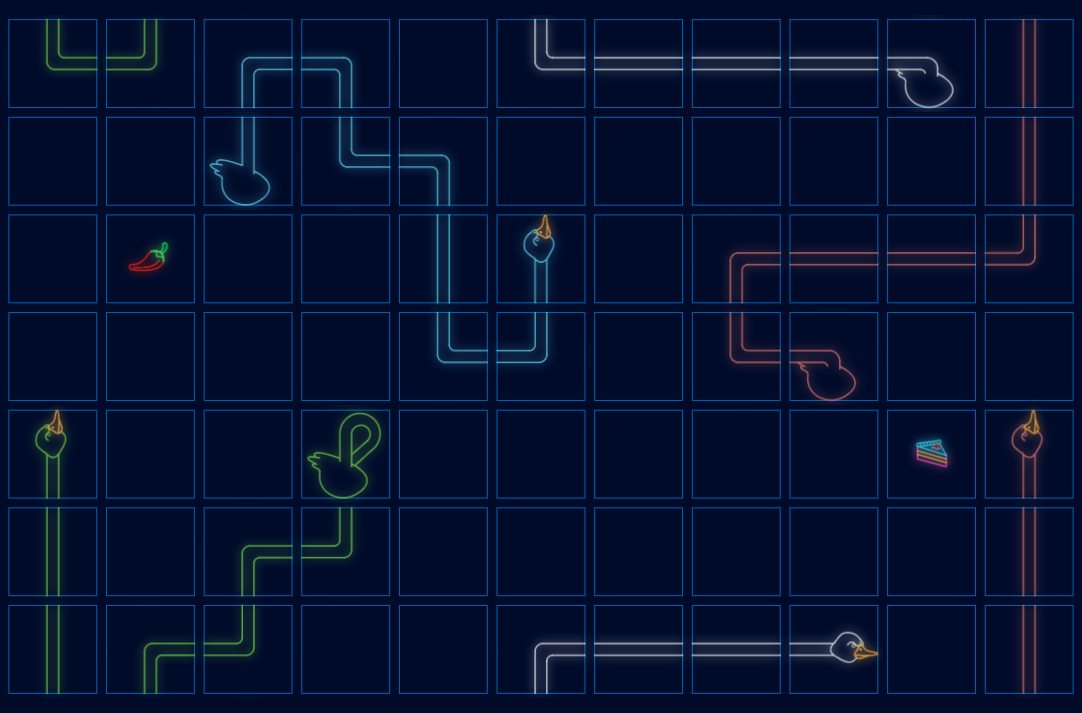
\includegraphics[width=\textwidth]{images/gameplay.png}
\caption{Gameplay Screenshot}
\label{figure_gameplay}
\end{figure}

Each goose will start with the length of one and they will spawn at a random location on the board. The game will run for a maximum of 200 turns or there is only one goose alive.

% The game board consists of 11 by 7 grid cells where each goose's body occupy a single cell \cite{game_rules}. This constrain the space in which the goose can move around. There can be up to 4 geese competing in the game. 

In each turn, each goose can choose to move up, down, left or right, relative to the orientation of the board. The goose is not allowed to take the opposite of its previous action even if the length of the goose is below three.

When the goose eats food, its length will increase by one. There is always two pieces of food on the board, and once a food is eaten, another food will spawn at a random unoccupied cell. At every 40 turns, the each goose will lose 1 segment of their body.

% During the each turn, each goose can choose to move in either NORTH, SOUTH, EAST, and WEST. They have a maximum time of 1 seconds to decide their movement. The geese can only move for 1 cell every turn and all their body parts will move simultaneously. Food such as donuts, pizza, pie or pepper will spawn randomly on unoccupied tiles. A maximum of two food can exists at any point of time. If a goose head collides with a food, it will increase its length by 1 and another food will spawn randomly. After 40 turns, all the geese will lose 1 segment of their body.

The primary objective of each goose is to survive to turn 200. Each goose is primarily ranked by the number of turns it survives. If two or more geese survive to turn 200, or die at the same time, the geese with the longer length will get a higher rank. The rank from each game will update the rating of the agent.

% If a goose's head collides with any goose's body, that goose will be eliminated and removed from the game. Also, any goose that loses their entire body will be eliminated.

% The game will end if 200 turns have passed and a score would be calculated for each goose participating. The higher the score, the better the rank of the goose's bot. The rank and the goose previous rating will determine the new rating.

\subsection{Competition Rules}
\label{subsection_competition}

The Kaggle competition started on January 26, 2021 and submission closes on July 21, 2021. Our team joined the competition late, making the first submission on June 23, 2021. Throughout the duration of the competition, each team can submit five agents every day, which will play against other agents. The team's placing in the competition is determined by the rating of the team's highest-rated agent.

Each agent will play against other agents of a similar rating. The magnitude of the change of rating will decrease as more games are played. After the close of the submissions, play between agents will continue to allow the agent rating to converge. The results are scheduled to be finalised on August 10, 2021, which is after the deadline of this report.

% No internet connection. Logs can be printed.

% Participants are also allowed to share their approaches publicly on Kaggle, in exchange for feedback and recognition.
% Somewhere in this section mention the point that you can submit the same models from another team. Teams may share their model while the submissions are still open. They do that to influence the competition to their own benefit, or for recognition with Kaggle promotion system, or to promote something else. All sharing between teams must be public.